%Version 3.1 December 2024
\documentclass[pdflatex, sn-nature]{sn-jnl}

%%%% Standard Packages
\usepackage{graphicx}%
\usepackage{multirow}%
\usepackage{amsmath,amssymb,amsfonts}%
\usepackage{amsthm}%
\usepackage{mathrsfs}%
\usepackage[title]{appendix}%
\usepackage{xcolor}%
\usepackage{textcomp}%
\usepackage{manyfoot}%
\usepackage{booktabs}%
\usepackage{algorithm}%
\usepackage{algorithmicx}%
\usepackage{algpseudocode}%
\usepackage{listings}%
\usepackage{siunitx}
\usepackage{cleveref}
%%%%

\graphicspath{{../Image/SI/}}

\crefname{figure}{Supplementary Figure}{Supplementary Figures}
\crefname{table}{Supplementary Table}{Supplementary Tables}
\crefname{section}{Supplementary Note}{Supplementary Notes}


\theoremstyle{thmstyleone}%
\newtheorem{theorem}{Theorem}%
\newtheorem{proposition}[theorem]{Proposition}% 

\theoremstyle{thmstyletwo}%
\newtheorem{example}{Example}%
\newtheorem{remark}{Remark}%

\theoremstyle{thmstylethree}%
\newtheorem{definition}{Definition}%

\setcounter{section}{0}
% \renewcommand{\thesection}{Supplementary Note \arabic{section}:}
\renewcommand{\thefigure}{S\arabic{figure}}
\renewcommand{\thetable}{S\arabic{table}}

\newcommand{\SupplementarySection}[1]{%
  \refstepcounter{section}%
  \section*{Supplementary Note \thesection: #1}%
  \addcontentsline{toc}{section}{Supplementary Note \thesection: #1}%
}

\raggedbottom


\begin{document}

\title[]{Supplementary Information for: Spatiotemporal Interference of Cutaneous Shear Waves Dictates Tactile Perception in Ultrasonic Haptics}

\author[1]{\fnm{Linhan} \sur{Fan}}\email{linhanfan@seu.edu.cn}

\author[1]{\fnm{Zhutao} \sur{Wang}}\email{xxxx@seu.edu.cn}

\author*[1]{\fnm{Yafeng} \sur{Niu}}\email{nyf@seu.edu.cn}

\affil*[1]{\orgdiv{School of Mechanical Engineering}, \orgname{Southeast University}, \orgaddress{\city{Nanjing}, \country{China}}}

\maketitle


\SupplementarySection{Backgrounds of the ultrasound phased array}







\SupplementarySection{Backgrounds of the ultrasound mid-air haptic}

Ultrasound mid-air haptics (UMH) technology enables the delivery of tactile feedback without physical contact by focusing airborne acoustic waves onto the skin surface~\cite{hoshiIntroductionUltrasonicMidair2022, rakkolainenSurveyMidAirUltrasound2021}. The underlying mechanism is acoustic radiation pressure, a non-linear effect arising from the momentum transfer of the acoustic field to an object~\cite{kingAcousticRadiationPressure1934a}. Given the large acoustic impedance mismatch between air and human skin ($\approx 99.9\%$), the incident ultrasound waves are almost entirely reflected, exerting a net force perpendicular to the skin surface~\cite{hoshiIntroductionUltrasonicMidair2022}. To generate perceptible forces, UMH systems utilize phased arrays of transducers to create constructive interference at specific spatial locations, forming a high-intensity acoustic focus~\cite{rakkolainenSurveyMidAirUltrasound2021, priceFibonacciSpiralArranged2018}.

Since the carrier frequency of these systems (typically \qty{40}{\kHz}) far exceeds the temporal sensitivity of cutaneous mechanoreceptors ($<\qty{1}{\kHz}$)~\cite{johnsonRolesFunctionsCutaneous2001, mountcastleNeuralBasisSense1967}, the acoustic field must be modulated to elicit tactile sensations. Amplitude Modulation (AM) varies the focal intensity at a perceptible frequency (e.g., \qty{200}{\Hz}) to activate Pacinian corpuscles~\cite{hoshiIntroductionUltrasonicMidair2022}. Alternatively, Spatiotemporal Modulation (STM) or Lateral Modulation (LM) rapidly steers the focal point along a trajectory on the skin~\cite{takahashiTactileStimulationRepetitive2020}. This scanning approach distributes the acoustic energy over a larger area and has been shown to generate shear shock waves in the skin, enhancing the perceived intensity and spatial extent of the tactile stimuli~\cite{reardonCutaneousWavePropagation2019, reardonShearShockWaves2023}.





\SupplementarySection{Ultrasound mid-air haptic device details}


\begin{figure}[htbp]
    \centering
    \includegraphics[width=\textwidth]{Figure_UMH_Device.pdf}
    \caption{\textbf{Overview of the custom-built Ultrasound Mid-Air Haptic (UMH) device.} \textbf{a}, Isometric view of the assembled device showing the compact hexagonal form factor. \textbf{b}, Top view of the acoustic aperture consisting of 60 ultrasonic transducers arranged in a hexagonal close-packed lattice with a central cutout for a CMOS sensor. \textbf{c}, Bottom view of the main control PCB, housing the STM32H750 microcontroller, USB-C data interface, and power management circuits. \textbf{d}, Side profile showing the USB-C data and debugging interfaces. \textbf{e}, Side profile showing the 12V DC power input jack. \textbf{f}, Bottom view of the transducer driver board. \textbf{g}, Detailed view of the driver circuitry for individual channels, highlighting the IX4428MTR driver ICs, TVS protection diodes, and status LEDs.}
    \label{fig:supplementary_figure_umh_device}
\end{figure}

\begin{figure}[htbp]
    \centering
    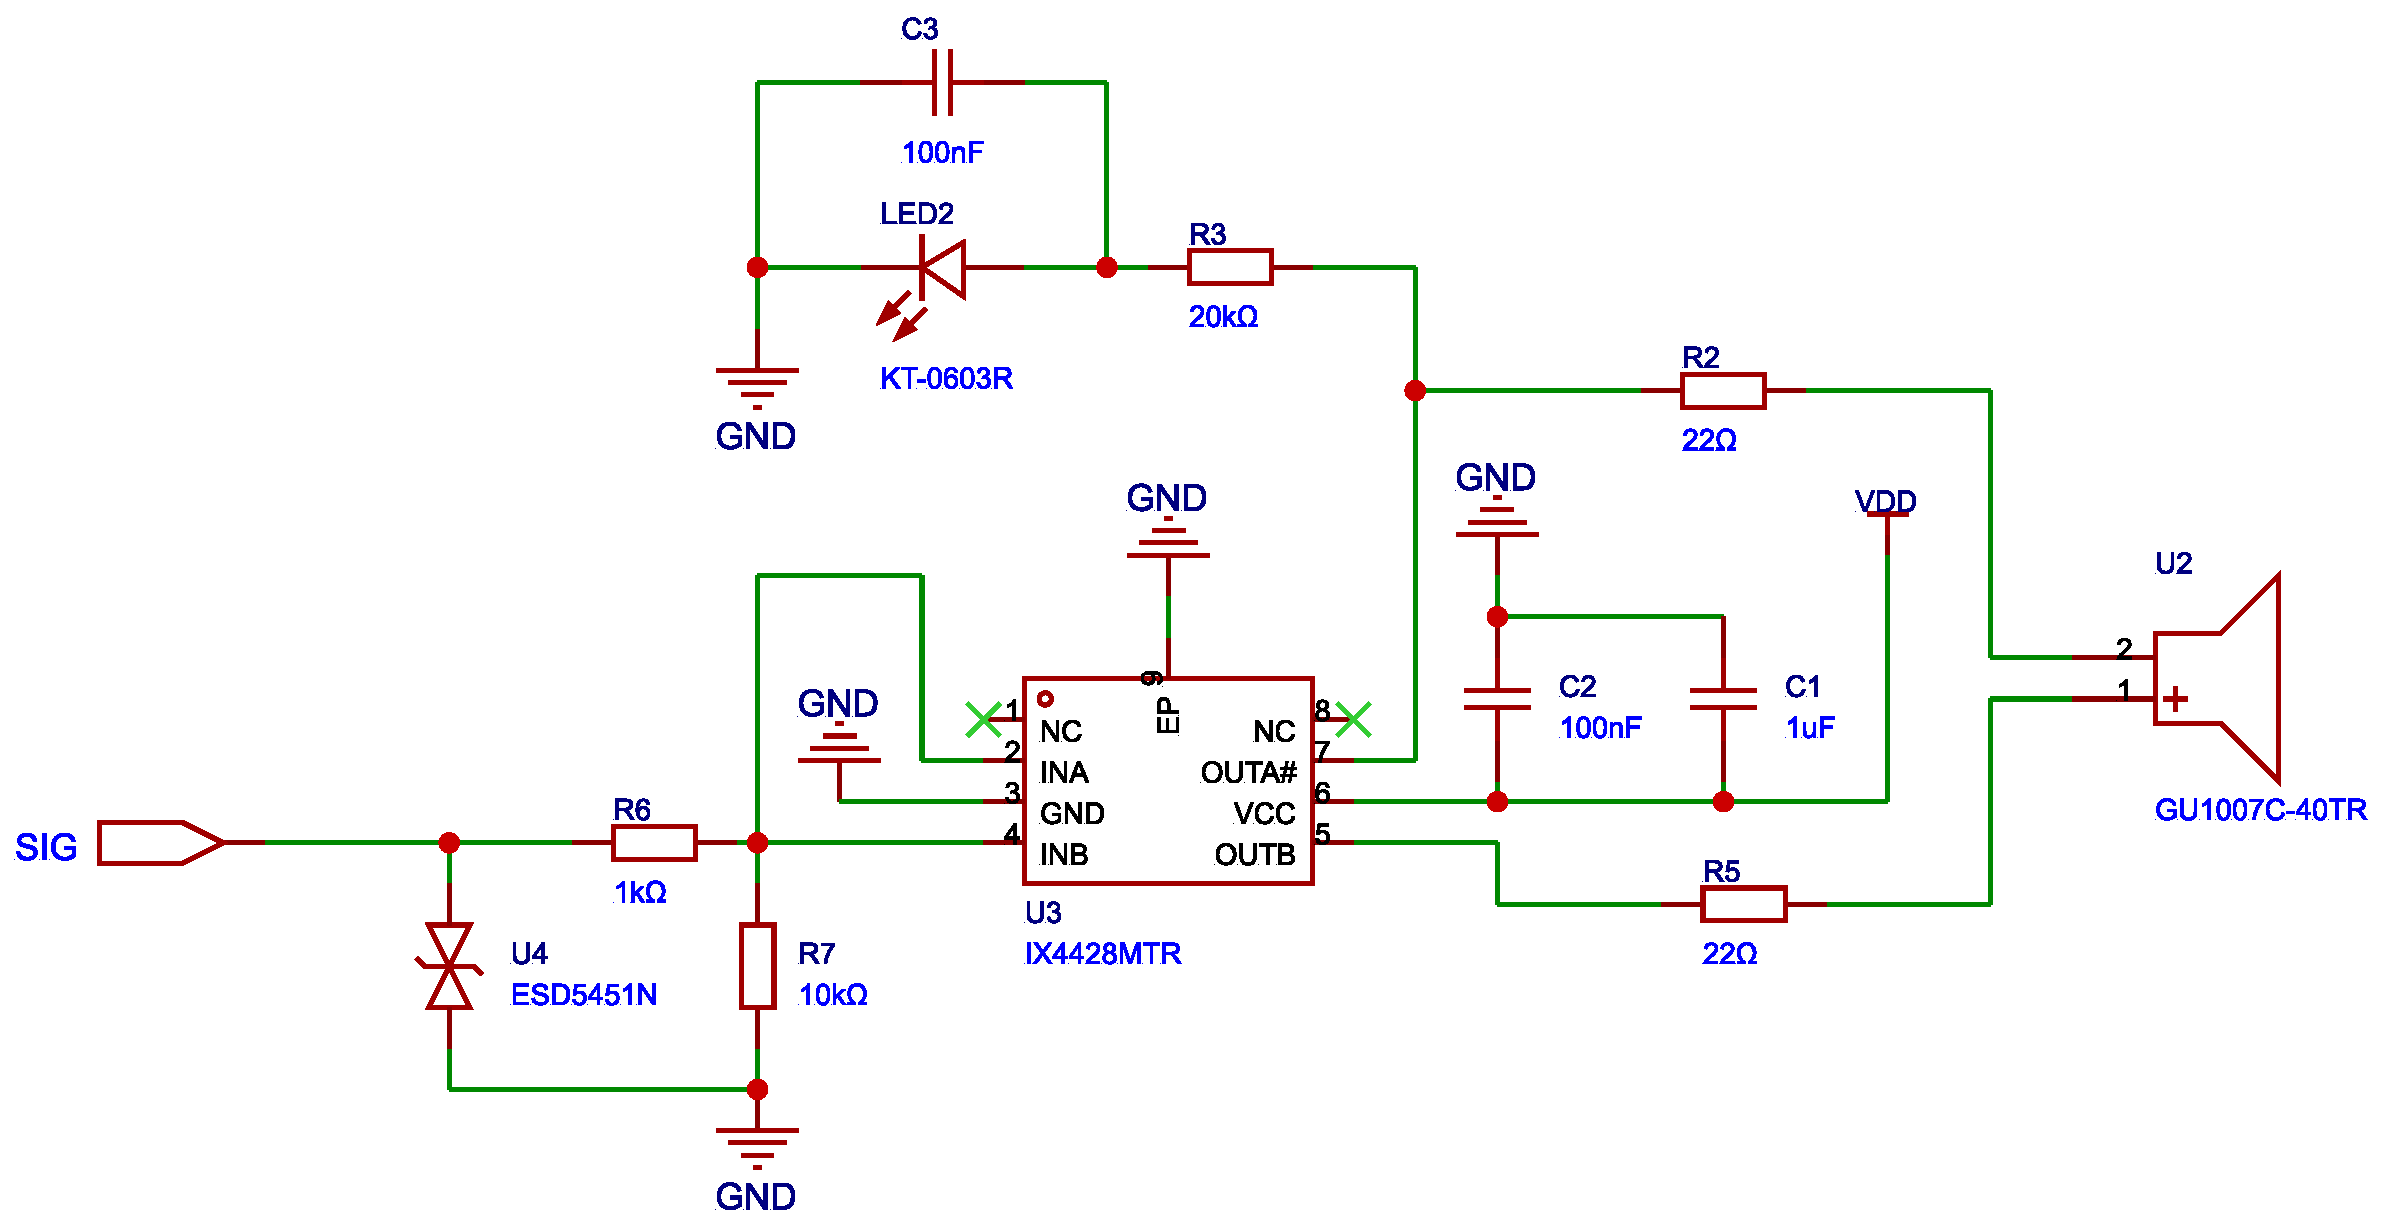
\includegraphics[width=\textwidth]{Figure_Transducer_Driver_Circuit.pdf}
    \caption{\textbf{Schematic of the single-channel ultrasonic transducer driver circuit.} The digital control signal (SIG) is buffered and inverted by the IX4428MTR driver IC to generate complementary outputs (OUTA and OUTB). This bipolar drive topology applies a \qty{24}{\volt} peak-to-peak square wave across the piezoelectric transducer (GU1007C-40TR) from a single \qty{12}{\volt} supply, maximizing acoustic emission. The circuit includes ESD protection and a visual status indicator.}
    \label{fig:supplementary_figure_transducer_driver_circuit}
\end{figure}


The experimental platform utilized in this study is a custom-developed, high-energy-density Ultrasound Mid-Air Haptic (UMH) device (\cref{fig:supplementary_figure_umh_device}a). The system integrates a phased array of ultrasonic transducers, multi-channel driving circuitry, and a central processing unit into a compact hexagonal prism form factor with dimensions of \qtyproduct{102.2 x 90 x 32.2}{\milli\meter}.


The acoustic aperture comprises 60 airborne ultrasonic transducers (GU1007C-40TR, Dongguan Ninghai Electronics Co., Ltd.) arranged in a hexagonal close-packed (HCP) lattice. The transducers have a diameter of \qty{10}{\milli\meter} and are spaced with a center-to-center pitch of \qty{10}{\milli\meter}, maximizing the fill factor for efficient acoustic power generation. A central aperture is reserved within the array to accommodate a CMOS image sensor for future visual tracking integration (\cref{fig:supplementary_figure_umh_device}b). Each transducer operates at a center frequency of \qty{40}{\kilo\hertz} with a directivity of approximately \ang{80}.

The device is powered by a \qty{12}{\volt} DC input, which is regulated to provide \qty{3.3}{\volt} and \qty{5.0}{\volt} rails for logic and analog subsystems. The core control unit is an STM32H750VBT6 microcontroller (STMicroelectronics) based on the ARM Cortex-M7 core. The MCU handles communication with the host PC via a USB Type-C interface using the CDC virtual serial port protocol.

To achieve precise phase control for beamforming, the system employs a Direct Memory Access (DMA) based signal generation mechanism. The MCU's timer triggers DMA transfers at a sampling frequency of \qty{4}{\mega\hertz}, updating the output state of the GPIO ports. For the \qty{40}{\kilo\hertz} carrier wave, each acoustic cycle is discretized into 100 time slices, providing a phase resolution of $2\pi/100$ (temporal resolution of \qty{250}{\nano\second}).

The amplification stage utilizes a bipolar drive topology to maximize the acoustic pressure output from the available \qty{12}{\volt} supply. As illustrated in the schematic (\cref{fig:supplementary_figure_transducer_driver_circuit}), the logic-level signal (SIG) is fed into a dual-channel low-side MOSFET driver (IX4428MTR, IXYS Integrated Circuits Division). The driver is configured to output two complementary square waves (OUTA and OUTB) to the transducer terminals. This push-pull configuration effectively doubles the voltage swing across the piezoelectric element to \qty{24}{\volt} peak-to-peak (Vpp). Each channel is equipped with a transient voltage suppressor (TVS) diode (ESD5451N) for electrostatic discharge protection and a status LED for visual monitoring of channel activity (\cref{fig:supplementary_figure_umh_device}g).


\begin{figure}[htbp]
    \centering
    \includegraphics[width=\textwidth]{Figure_Transducer_Array_Arrangement_Focus_Simulation_Results.png}
    \caption{\textbf{Comparative simulation of acoustic focusing performance across different transducer array layouts.} The four rows correspond to (from top to bottom): Hexagonal Close-Packed ($N=60$), Rectangular ($N=64$), Density-Tapered Vogel Spiral ($N=60$), and Optimized Fermat Spiral ($N=60$). The columns display: (Left) The array geometry and physical footprint; (Middle) The normalized acoustic pressure distribution on the focal plane ($z=\qty{100}{\milli\meter}$), annotated with the Area-based Array Performance Index ($\text{API}_{area}$) and maximum pressure; (Right) The side-view pressure distribution in the XZ plane, annotated with the Volume-based Array Performance Index ($\text{API}_{vol}$). The hexagonal array (top row) offers the optimal balance of high pressure output and compact size for the proposed device.}
    \label{fig:supplementary_figure_transducer_array_arrangement_focus_simulation_results}
\end{figure}

To systematically evaluate the acoustic performance of the chosen hexagonal transducer arrangement and explore potential optimizations for future iterations, we conducted comparative numerical simulations of four distinct phased array configurations. The simulation model utilized the Rayleigh-Sommerfeld integral to calculate the acoustic pressure field generated by circular piston sources ($d=\qty{10}{\milli\meter}$) operating at \qty{40}{\kilo\hertz} in air ($c=\qty{343}{\meter\per\second}$). The configurations included: (1) the proposed Hexagonal Close-Packed (HCP) array ($N=60$, Area=\qty{54.4}{\centi\meter\squared}), (2) a standard Rectangular grid ($N=64$, Area=\qty{63.8}{\centi\meter\squared}), (3) a Density-Tapered Vogel Spiral ($N=60$, Area=\qty{102.7}{\centi\meter\squared}), and (4) an Optimized Fermat Spiral ($N=60$, Area=\qty{104.1}{\centi\meter\squared}).

The geometric arrangement of transducers significantly influences the beamforming capabilities. For the periodic arrays, the Rectangular layout follows a standard Cartesian grid, while the Hexagonal Close-Packed (HCP) coordinates are derived from the triangular lattice vectors defined by:
\begin{equation}
    x_{q,r} = d \left(q + \frac{r}{2}\right), \quad y_{q,r} = d \frac{\sqrt{3}}{2} r
\end{equation}
where $d=\qty{10}{\milli\meter}$ is the pitch and $q, r$ are integers. This hexagonal arrangement maximizes the surface fill factor. In contrast, the aperiodic spiral arrays utilize the golden angle $\Phi_g = \pi(3-\sqrt{5}) \approx \ang{137.5}$ to suppress grating lobes. The Optimized Fermat Spiral places the $n$-th element at $\theta_n = n \Phi_g$ and radial distance $r_n = c \sqrt{n} (1 + \beta n)$, where the term $(1 + \beta n)$ introduces a radial density taper to reduce side lobes. The Density-Tapered Vogel Spiral is generated using an iterative collision-based packing algorithm, where the exclusion radius for the $n$-th element expands linearly as $d_{req}(n) = d_{min}(1 + \alpha n)$, creating a spatially apodized aperture that transitions from a dense core to a sparse periphery.

The focusing performance was quantified using the Array Performance Index (API) \cite{priceFibonacciSpiralArranged2018, holmesPostprocessingFullMatrix2005}, a dimensionless metric defined for both the focal area and volume. The area-based API is calculated as $\text{API}_{area} = A_{-6dB} / \lambda^2$, where $A_{-6dB}$ represents the area within the \qty{-6}{\decibel} pressure contour on the focal plane. Similarly, the volume-based API is defined as $\text{API}_{vol} = V_{-6dB} / \lambda^3$, capturing the spatial confinement of the acoustic energy. A lower API value indicates sharper focusing and superior diffraction-limited performance.

As illustrated in \cref{fig:supplementary_figure_transducer_array_arrangement_focus_simulation_results}, the spiral configurations demonstrate superior focusing characteristics with significantly lower API values ($\text{API}_{area} \approx 1.65-1.89$) and suppressed grating lobes compared to the periodic arrays. However, their sparse arrangement results in a larger physical footprint and reduced peak pressure output ($\approx \qty{540}{\pascal}$) for the same element count. Conversely, the proposed hexagonal array achieves a high peak pressure of \qty{581}{\pascal} with a compact footprint, leveraging the maximum packing density. Although it exhibits characteristic hexagonal grating lobes and a slightly higher API ($\text{API}_{area} = 2.57$), the focal quality remains sufficient for precise tactile stimulation. Consequently, the hexagonal layout was selected for the current prototype to maximize acoustic power density within a handheld form factor, while the spiral designs provide a validated pathway for future high-fidelity, large-aperture applications.



\SupplementarySection{Psychophysical experimental details}

Experiment~1 was designed as a within-participant paired-comparison psychophysical study to resolve perceptual differences among five ultrasonic spatiotemporal modulation strategies under weak near-threshold tactile conditions. The five tested stimuli were 
$DLM_2$, $DLM_3$, $ULM_L$, $LM_L$, and $LM_C$, corresponding respectively to two-point discrete lateral modulation, three-point discrete lateral modulation, unidirectional linear lateral modulation, bidirectional linear lateral modulation, and continuous circular lateral modulation. We selected a forced-comparison design because absolute ratings are unstable when the tactile magnitude of each individual ultrasonic stimulus is small and because paired judgments provide higher sensitivity for detecting relative perceptual ordering~\citep{bradleyRankAnalysisIncomplete1952, johnsonNeuralBasisHaptic2002}. The experiment therefore aimed to estimate relative perceptual dominance rather than absolute magnitude.

All stimulation was delivered with the custom UMH device described above. The carrier frequency of the phased array was \qty{40}{\kilo\hertz}, whereas the tactile modulation frequency was fixed at \qty{200}{\hertz}, a range strongly coupled to the Pacinian-dominant vibrotactile channel of glabrous skin~\citep{mountcastleNeuralBasisSense1967, talbotSenseFluttervibrationComparison1968a, johnsonRolesFunctionsCutaneous2001, handlerMechanosensoryNeuronsTouch2021}. Participants placed the palm on a foam support that fixed the hand-device distance and reduced posture-dependent variability in acoustic coupling. They wore noise-cancelling headphones continuously playing white noise so that judgments relied on cutaneous sensation rather than on airborne acoustic leakage or switching sounds from the phased array. These controls were critical because several modulation methods, especially the discrete switching conditions, can generate audible artifacts that might otherwise provide non-tactile cues.

The five stimuli were parameterized around a common focal center at $(0,0,\qty{0.1}{\meter})$. The modulation frequency was fixed at $f=\qty{200}{\hertz}$, giving a period of
\begin{equation}
T = \frac{1}{f} = \qty{5}{\milli\second} .
\end{equation}
Trajectory geometry was chosen from the assumed cutaneous shear-wave speed $c_s=\qty{5}{\meter\per\second}$ so that the programmed focal transition times or scan velocities approximately matched the propagation timescale of surface waves. For $DLM_2$, the focal points lay on a ring of radius $R_{2}=\qty{6.25}{\milli\meter}$, so that the distance between the two diametrically opposed points was $2R_{2}=\qty{12.5}{\milli\meter}=c_sT/2$. For $DLM_3$, the focal points formed an equilateral triangle on a ring of radius $R_{3}=\qty{4.81}{\milli\meter}$, such that the adjacent-point spacing satisfied $\sqrt{3}R_{3}\approx \qty{8.33}{\milli\meter}=c_sT/3$. For $ULM_L$, the focus traversed a unidirectional linear path of length $L_{U}=\qty{30}{\milli\meter}$ in each period, yielding an effective scan speed
\begin{equation}
v_U = \frac{L_U}{T} = \qty{6}{\meter\per\second} \approx 1.2\,c_s .
\end{equation}
For $LM_L$, the focus moved bidirectionally between two endpoints separated by \qty{15}{\milli\meter}; because the focus covered the outbound and return paths within one modulation period, the total travelled distance per period was \qty{30}{\milli\meter}, again corresponding to an average path speed of \qty{6}{\meter\per\second}. For $LM_C$, the focus moved continuously along a circular trajectory of radius $R_C=\qty{4.77}{\milli\meter}$, for which the tangential speed was set to the same Mach number regime, $v_C\approx \qty{6}{\meter\per\second} \approx 1.2\,c_s$. Matching the nominal kinematic scale across conditions reduced confounding by trivial differences in scan frequency or gross path length and focused the comparison on how different spatiotemporal wave organizations shape perception.

The experiment contained two task blocks. In the Intensity block, participants reported which of two successively presented stimuli felt stronger. In the Spatial block, participants reported which stimulus felt smaller or clearer as a tactile point. We retained the label ``smaller / clearer'' because the task was intended to capture the perceptual sharpness of a localized tactile percept under weak ultrasonic stimulation, rather than physical spatial acuity in the strict classical two-point-discrimination sense. This distinction is important because, under near-threshold conditions, judgments of ``clarity'' likely integrate perceived detectability, compactness, temporal stability, and confidence in addition to apparent stimulus area.

The two task blocks were presented in randomized order for each participant. Within each block, the five stimuli generate $\binom{5}{2}=10$ unordered pairs. To control for first-versus-second presentation effects, every unordered pair was presented in both temporal orders, yielding $5\times4=20$ ordered trials per block. The trial list was therefore the complete set of ordered permutations of length two over the five stimuli. Trial order was then shuffled independently within each block. Because the block order was also randomized, each participant completed a total of 40 forced-choice trials. During data collection, the graphical user interface concealed the identities of the current stimulus pair from both participant and experimenter during trial execution, thereby implementing an operationally blind procedure at the level of stimulus identity display.

Each trial followed a fixed temporal structure. Stimulus~A was presented for \qty{1.5}{\second}, followed by a silent interval of \qty{1.0}{\second}, after which Stimulus~B was presented for \qty{1.5}{\second}. The silent interval was introduced to reduce immediate peripheral and central carry-over from the first stimulus while keeping the comparison in short-term tactile memory. Replay was not allowed. Participants had to commit to a first-pass comparative judgment, which is consistent with standard two-alternative forced-choice logic and avoids strategic averaging across repeated presentations~\citep{bradleyRankAnalysisIncomplete1952}. The response was recorded only after the second stimulus ended. Reaction time was measured from the offset of Stimulus~B to the submission of the response, so the recorded decision time indexed post-stimulus comparative evaluation rather than motor latency during stimulation.

Responses were stored trial-by-trial in comma-separated files, with one file per participant. Each record contained the participant identifier, timestamp, block index, block type, trial number, stimulus identity in the first and second positions, the selected winner for the active judgment dimension, and reaction time. Because each block queried only one perceptual dimension, the non-relevant response field for that trial was left empty. This structure preserved the full order information required for paired-comparison modeling while keeping intensity and spatial judgments analytically separable.

A priori sample-size estimation was carried out in G*Power using an effect size of $g=0.2$, $\alpha=0.05$, power $=0.8$, and constant proportion $=0.5$, which yielded a required total sample size of 49 paired observations at the comparison level. Because each participant contributed both presentation orders for a given unordered pair, this requirement corresponded to approximately 25 participants. We therefore recruited 30 participants for Experiment~1, with a balanced sex distribution (15 male and 15 female), to provide a margin against data loss and to stabilize estimation of individual differences in the mixed-effects analysis.

The primary analysis treated paired choices as comparative preference data and modeled them with a Bayesian mixed-effects Bradley--Terry framework~\citep{bradleyRankAnalysisIncomplete1952}. For each block, the raw trial table was converted into long format, with one row per valid paired comparison. Let stimuli $i$ and $j$ denote the first and second members of a presented pair for a given trial, and let $Y_{n}=1$ if stimulus $i$ was chosen over stimulus $j$ on trial $n$, and $Y_{n}=0$ otherwise. The probability that stimulus $i$ defeats stimulus $j$ was modeled as
\begin{equation}
\Pr(Y_n=1)=\frac{\exp\left(\lambda_i-\lambda_j+b_{p[n]}\right)}{1+\exp\left(\lambda_i-\lambda_j+b_{p[n]}\right)} ,
\end{equation}
where $\lambda_i$ and $\lambda_j$ are fixed-effect latent scores for the two modulation methods and $b_{p[n]}$ is the participant-specific random intercept for the participant $p[n]$ who generated trial $n$. In implementation, the model was estimated using a binomial Bayesian mixed generalized linear model, with participant identity entered as a random effect. After fitting, the estimated method scores were mean-centered,
\begin{equation}
\tilde{\lambda}_i = \lambda_i - \frac{1}{K}\sum_{k=1}^{K}\lambda_k,
\end{equation}
where $K=5$ is the number of modulation methods. This zero-centered representation preserves all pairwise contrasts while making the average method score equal to zero, which simplifies visual comparison between methods and between task blocks.

For descriptive inspection before model fitting, we constructed a win matrix for each block. Its $(i,j)$ element counted the number of trials on which method $i$ was chosen over method $j$. The win matrix provides an intuitive summary of pairwise dominance structure, but inferential conclusions were based on the mixed-effects Bradley--Terry estimates and their covariance. Pairwise contrasts between methods were evaluated using Wald statistics derived from the fitted score covariance matrix. For a contrast between methods $i$ and $j$, we computed
\begin{equation}
\Delta_{ij}=\tilde{\lambda}_i-\tilde{\lambda}_j,
\qquad
z_{ij}=\frac{\Delta_{ij}}{\sqrt{\mathrm{Var}(\Delta_{ij})}},
\end{equation}
with two-sided $p$ values obtained from the standard normal distribution. We also report the corresponding odds ratio,
\begin{equation}
\mathrm{OR}_{ij}=\exp(\Delta_{ij}),
\end{equation}
which quantifies the multiplicative advantage of method $i$ over method $j$ in the paired-comparison choice probability. Statistical significance was annotated using the conventional thresholds $p<0.05$, $p<0.01$, and $p<0.001$.

We analyzed decision time as a secondary marker of discriminability. Longer decisions were interpreted as indicating smaller perceptual distances between the two methods being compared. Reaction times shorter than \qty{0.2}{\second} or longer than \qty{10}{\second} were treated as invalid and excluded from this analysis. For the remaining trials, raw reaction time $RT$ was natural-log transformed to reduce right skew,
\begin{equation}
\mathrm{LogRT}=\ln(RT),
\end{equation}
and then standardized within participant to remove idiosyncratic baseline response speed,
\begin{equation}
Z\mathrm{LogRT}_{n}=\frac{\mathrm{LogRT}_{n}-\mu_{p[n]}}{\sigma_{p[n]}} ,
\end{equation}
where $\mu_{p[n]}$ and $\sigma_{p[n]}$ are the participant-specific mean and standard deviation of log reaction time. Trials from participants with zero or undefined within-participant variance were assigned a standardized value of zero in the implementation. We then averaged $Z\mathrm{LogRT}$ across all presentations of each unordered stimulus pair to form a symmetric reaction-time matrix. Darker values in the corresponding heat map indicate longer normalized decisions and, by inference, smaller perceptual separation between the two compared stimuli.

Visualization followed the structure of the statistical analysis. For the Intensity and Spatial blocks, each method was displayed as a bar whose height represented the centered Bradley--Terry score, with error bars corresponding to the 
\qty{95}{\percent} confidence interval approximated as $\pm 1.96\times SE$. Significant pairwise contrasts were marked directly on the plots. Reaction-time results were summarized as a stimulus-by-stimulus heat map of mean standardized log reaction time. Together, these visualizations allowed us to compare perceptual rank order, uncertainty, pairwise separability, and decision difficulty within a single coherent analytical framework.

The principal findings, taken directly from the finalized analysis reported in the project record, were as follows. In the Intensity block, $ULM_L$ achieved the highest centered Bradley--Terry score ($0.74\pm0.11$), followed by $DLM_2$ ($0.34\pm0.11$), $DLM_3$ ($-0.04\pm0.11$), $LM_C$ ($-0.18\pm0.11$), and $LM_L$ ($-0.86\pm0.12$). $ULM_L$ was significantly preferred over every other method, and $LM_L$ performed worst overall. In the Spatial block, $ULM_L$ again showed the highest score ($0.24\pm0.10$), followed by $DLM_2$ ($0.11\pm0.10$), $DLM_3$ ($-0.04\pm0.10$), $LM_C$ ($-0.08\pm0.10$), and $LM_L$ ($-0.23\pm0.10$). However, spatial judgments were less strongly separated than intensity judgments, and only a subset of pairwise contrasts reached significance. Reaction-time analysis showed that decisions were slowest for pairs such as $DLM_3$ versus $LM_C$ and $ULM_L$ versus $DLM_2$, consistent with the close perceptual proximity of those pairs in the Bradley--Terry score space. By contrast, comparisons involving $LM_L$ were typically faster, consistent with its relatively poor perceptual performance and therefore easier exclusion in forced-choice decisions.

These psychophysical observations informed the later mechanistic interpretation of the study. Most importantly, the results show that perceptual superiority did not follow a simple expectation based on static focal intensity or geometric sharpness alone. Instead, the best-performing condition was the one that preserved the intended \qty{200}{\hertz} temporal structure while organizing cutaneous shear-wave propagation into a more coherent spatiotemporal pattern. The psychophysical protocol was therefore explicitly constructed not merely to rank five engineering implementations, but to provide a sensitive behavioral assay of how modulation-dependent wave organization shapes tactile perception in ultrasonic haptics.

\SupplementarySection{Numerical Simulation of Tactile Wave Propagation}

Numerical simulations were conducted to investigate the propagation characteristics of tactile stimuli in soft tissue under different modulation schemes. We performed these simulations using the k-Wave toolbox in MATLAB R2025b (The MathWorks Inc., Natick, MA, USA), specifically utilizing the \texttt{pstdElastic3D} solver to model elastic wave propagation in isotropic, heterogeneous media.

The simulation domain represented a human skin tissue volume with dimensions of \qtyproduct{80 x 80 x 40}{\milli\meter}. The computational grid was discretized with a spatial step size of $dx = dy = dz = \qty{1.0}{\milli\meter}$. The medium properties represented human soft tissue:
\begin{itemize}
    \item Density: $\rho = \qty{923.5}{\kilo\gram\per\cubic\meter}$.
    \item Shear wave speed: $c_s = \qty{5.0}{\meter\per\second}$.
    \item Compressional wave speed: $c_p = \qty{100}{\meter\per\second}$. Although the physical speed of sound in soft tissue is approximately \qty{1540}{\meter\per\second}, we used a reduced value to improve computational efficiency. This satisfies the condition $c_p \gg c_s$ without affecting the shear wave dynamics that dominate tactile perception.
    \item Shear wave attenuation: $\alpha_s = \qty{10}{\decibel\per\mega\hertz\squared\per\centi\meter}$ (power law exponent $y=2.0$).
    \item Compressional wave attenuation: $\alpha_p = \qty{0.1}{\decibel\per\mega\hertz\tothe{1.5}\per\centi\meter}$ (power law exponent $y=1.5$).
\end{itemize}

A Perfectly Matched Layer (PML) applied to the lateral and bottom boundaries simulated a semi-infinite medium to eliminate boundary reflections. Additionally, we added a sponge layer (20 grid points) with a quadratic absorption profile to the bottom boundary.

The tactile stimulus was modeled as a vertical stress source $S_{zz}$ at the skin surface ($z=0$), representing the acoustic radiation force generated by focused ultrasound. The source is defined by the spatiotemporal function:
\begin{equation}
    S_{zz}(x, y, t) = A(t) \cdot S_0 \cdot \exp\left(-\frac{(x - x_f(t))^2 + (y - y_f(t))^2}{2\sigma^2}\right)
\end{equation}

where $S_0 = \qty{100}{\pascal}$ is the peak stress amplitude, and $\sigma = \qty{4.25}{\milli\meter}$ defines the spatial width of the focal point. The temporal modulation $A(t)$ was a continuous \qty{200}{\hertz} sine wave with a duration of \qty{75}{\milli\second} (15 cycles). The focal point trajectory $(x_f(t), y_f(t))$ varied according to the five modulation methods. Geometric parameters for these trajectories were determined based on the modulation frequency ($f = \qty{200}{\hertz}$, period $T = \qty{5}{\milli\second}$) and the skin shear wave speed ($c_s = \qty{5.0}{\meter\per\second}$), ensuring that focal point movement or switching generally matched natural wave propagation characteristics:

\begin{enumerate}
    \item \textbf{DLM-2 (Discrete Lateral Modulation - 2 Points):} The focus alternates between two discrete points on a circle of radius $R=\qty{6.25}{\milli\meter}$. This radius ensures the wave propagation time between the two points (distance $2R$) equals half the modulation period ($T/2$), satisfying $2R = c_s \cdot (T/2)$.
    \item \textbf{DLM-3 (Discrete Lateral Modulation - 3 Points):} The focus alternates among three discrete points on a circle of radius $R=\qty{4.81}{\milli\meter}$. This radius ensures the wave propagation time between adjacent points (distance $\sqrt{3}R$) equals one-third of the modulation period ($T/3$), satisfying $\sqrt{3}R = c_s \cdot (T/3)$.
    \item \textbf{ULM-L (Uniform Lateral Modulation - Line):} The focus scans linearly in one direction along a path of length $L=\qty{30}{\milli\meter}$. This corresponds to a scanning speed of $v = \qty{6.0}{\meter\per\second}$, slightly higher than the shear wave speed.
    \item \textbf{LM-L (Lateral Modulation - Line)~\citep{takahashiTactileStimulationRepetitive2020}:} The focus scans back and forth linearly along a path of length $L=\qty{15}{\milli\meter}$. This corresponds to an average scanning speed of $v = \qty{6.0}{\meter\per\second}$ (covering distance $2L$ in one period).
    \item \textbf{LM-C (Lateral Modulation - Circle)~\citep{takahashiTactileStimulationRepetitive2020}:} The focus moves continuously along a circular path of radius $R=\qty{4.77}{\milli\meter}$. This corresponds to a circumferential scanning speed of approximately $v = \qty{6.0}{\meter\per\second}$.
\end{enumerate}

Simulation output was recorded at a depth of \qty{1}{\milli\meter} below the surface. We analyzed the stress tensor components ($\tau_{xy}, \tau_{xz}, \tau_{yz}$) to evaluate tactile sensation intensity and spatial distribution. Key metrics included:

\begin{itemize}
    \item \textbf{RMS Stress Map:} The root-mean-square value of the stress magnitude over the last cycle of the steady-state period, representing the average energy distribution.
    \item \textbf{Peak Stress Map:} The maximum instantaneous stress magnitude recorded during the simulation.
    \item \textbf{Maximum Stress Rate Map:} The maximum time derivative of the stress magnitude ($\max |\partial |\boldsymbol{\tau}| / \partial t|$), indicating the dynamic intensity of the tactile stimulus.
    \item \textbf{Spatial Gradient:} The magnitude of the spatial gradient of the stress field at the final time step, providing cues for spatial resolution.
\end{itemize}

To ensure fair comparison between different modulation methods and accurate presentation of wavefield characteristics, the following key processing methods were adopted:
\begin{itemize}
    \item \textbf{Global Normalization and Colormaps:} To facilitate direct visual comparison of relative intensities across the five modulation methods, a unified color scale was applied to each scalar field metric. The upper limit of the color scale was fixed to the global maximum value found across all simulation groups. For positive-definite quantities, including the RMS shear stress magnitude ($|\boldsymbol{\tau}|_{\text{RMS}}$), peak shear stress magnitude ($|\boldsymbol{\tau}|_{\text{peak}}$), and maximum stress rate ($|\partial |\boldsymbol{\tau}| / \partial t|$), the perceptually uniform `inferno' colormap was utilized to represent intensity variations.
    \item \textbf{Spectrum Analysis Preprocessing:} The frequency content was analyzed based on the temporal waveform of the shear stress magnitude $|\boldsymbol{\tau}|(t)$ extracted at the geometric focus. To ensure accurate spectral estimation, the time-domain signal (length $L$) was first demeaned to remove the DC offset inherent to the magnitude calculation. A Hann window was then applied to minimize spectral leakage. To enhance the frequency resolution of the Fast Fourier Transform (FFT), the signal was zero-padded to a length of $N_{FFT} = 2^{\lceil \log_2(8L) \rceil}$. The resulting magnitude spectrum was converted to the decibel (dB) scale for display.
    \item \textbf{Spatiotemporal (XT) Diagram:} To visualize the wave propagation dynamics and interference patterns, we extracted the signed shear stress component $\tau_{xz}$ along the lateral axis ($y=0$). The time-domain signal at each spatial point was processed by subtracting its temporal mean to remove the static background stress, thereby highlighting the dynamic fluctuations. The resulting spatiotemporal map was plotted using a diverging colormap (`RdBu\_r') to distinguish between positive and negative shear phases.
    \item \textbf{Instantaneous Wavefront Snapshots:} The transient evolution of the wavefield was captured by extracting the shear stress component $\tau_{xy}$ at four distinct phase points ($T/4, T/2, 3T/4, T$) within the first excitation cycle. Each snapshot was spatially demeaned to center the colormap range, ensuring that the polarity of the shear waves was clearly visualized using a diverging colormap (`RdBu\_r').
    \item \textbf{Focusing Performance Evaluation:} The spatial focusing resolution was quantified using the lateral distribution of the peak shear stress magnitude $|\boldsymbol{\tau}|_{\text{peak}}$ on the focal plane. The stress profile was normalized to its maximum value, and the Full Width at Half Maximum (FWHM) was calculated by determining the spatial width where the normalized intensity exceeded 0.5.
\end{itemize}

\cref{fig:supplementary_figure_sim_1_full_spatial} and \cref{fig:supplementary_figure_sim_1_full_temporal} present the comprehensive simulation results for the five modulation schemes. \cref{fig:supplementary_figure_sim_1_full_spatial} visualizes the spatial distribution of the key stress metrics, allowing for a direct comparison of the stimulated area and intensity patterns. \cref{fig:supplementary_figure_sim_1_full_temporal} details the temporal evolution of the wavefields, illustrating the dynamic propagation characteristics and the resulting waveforms at the focal center.

\begin{figure}[htbp]
    \centering
    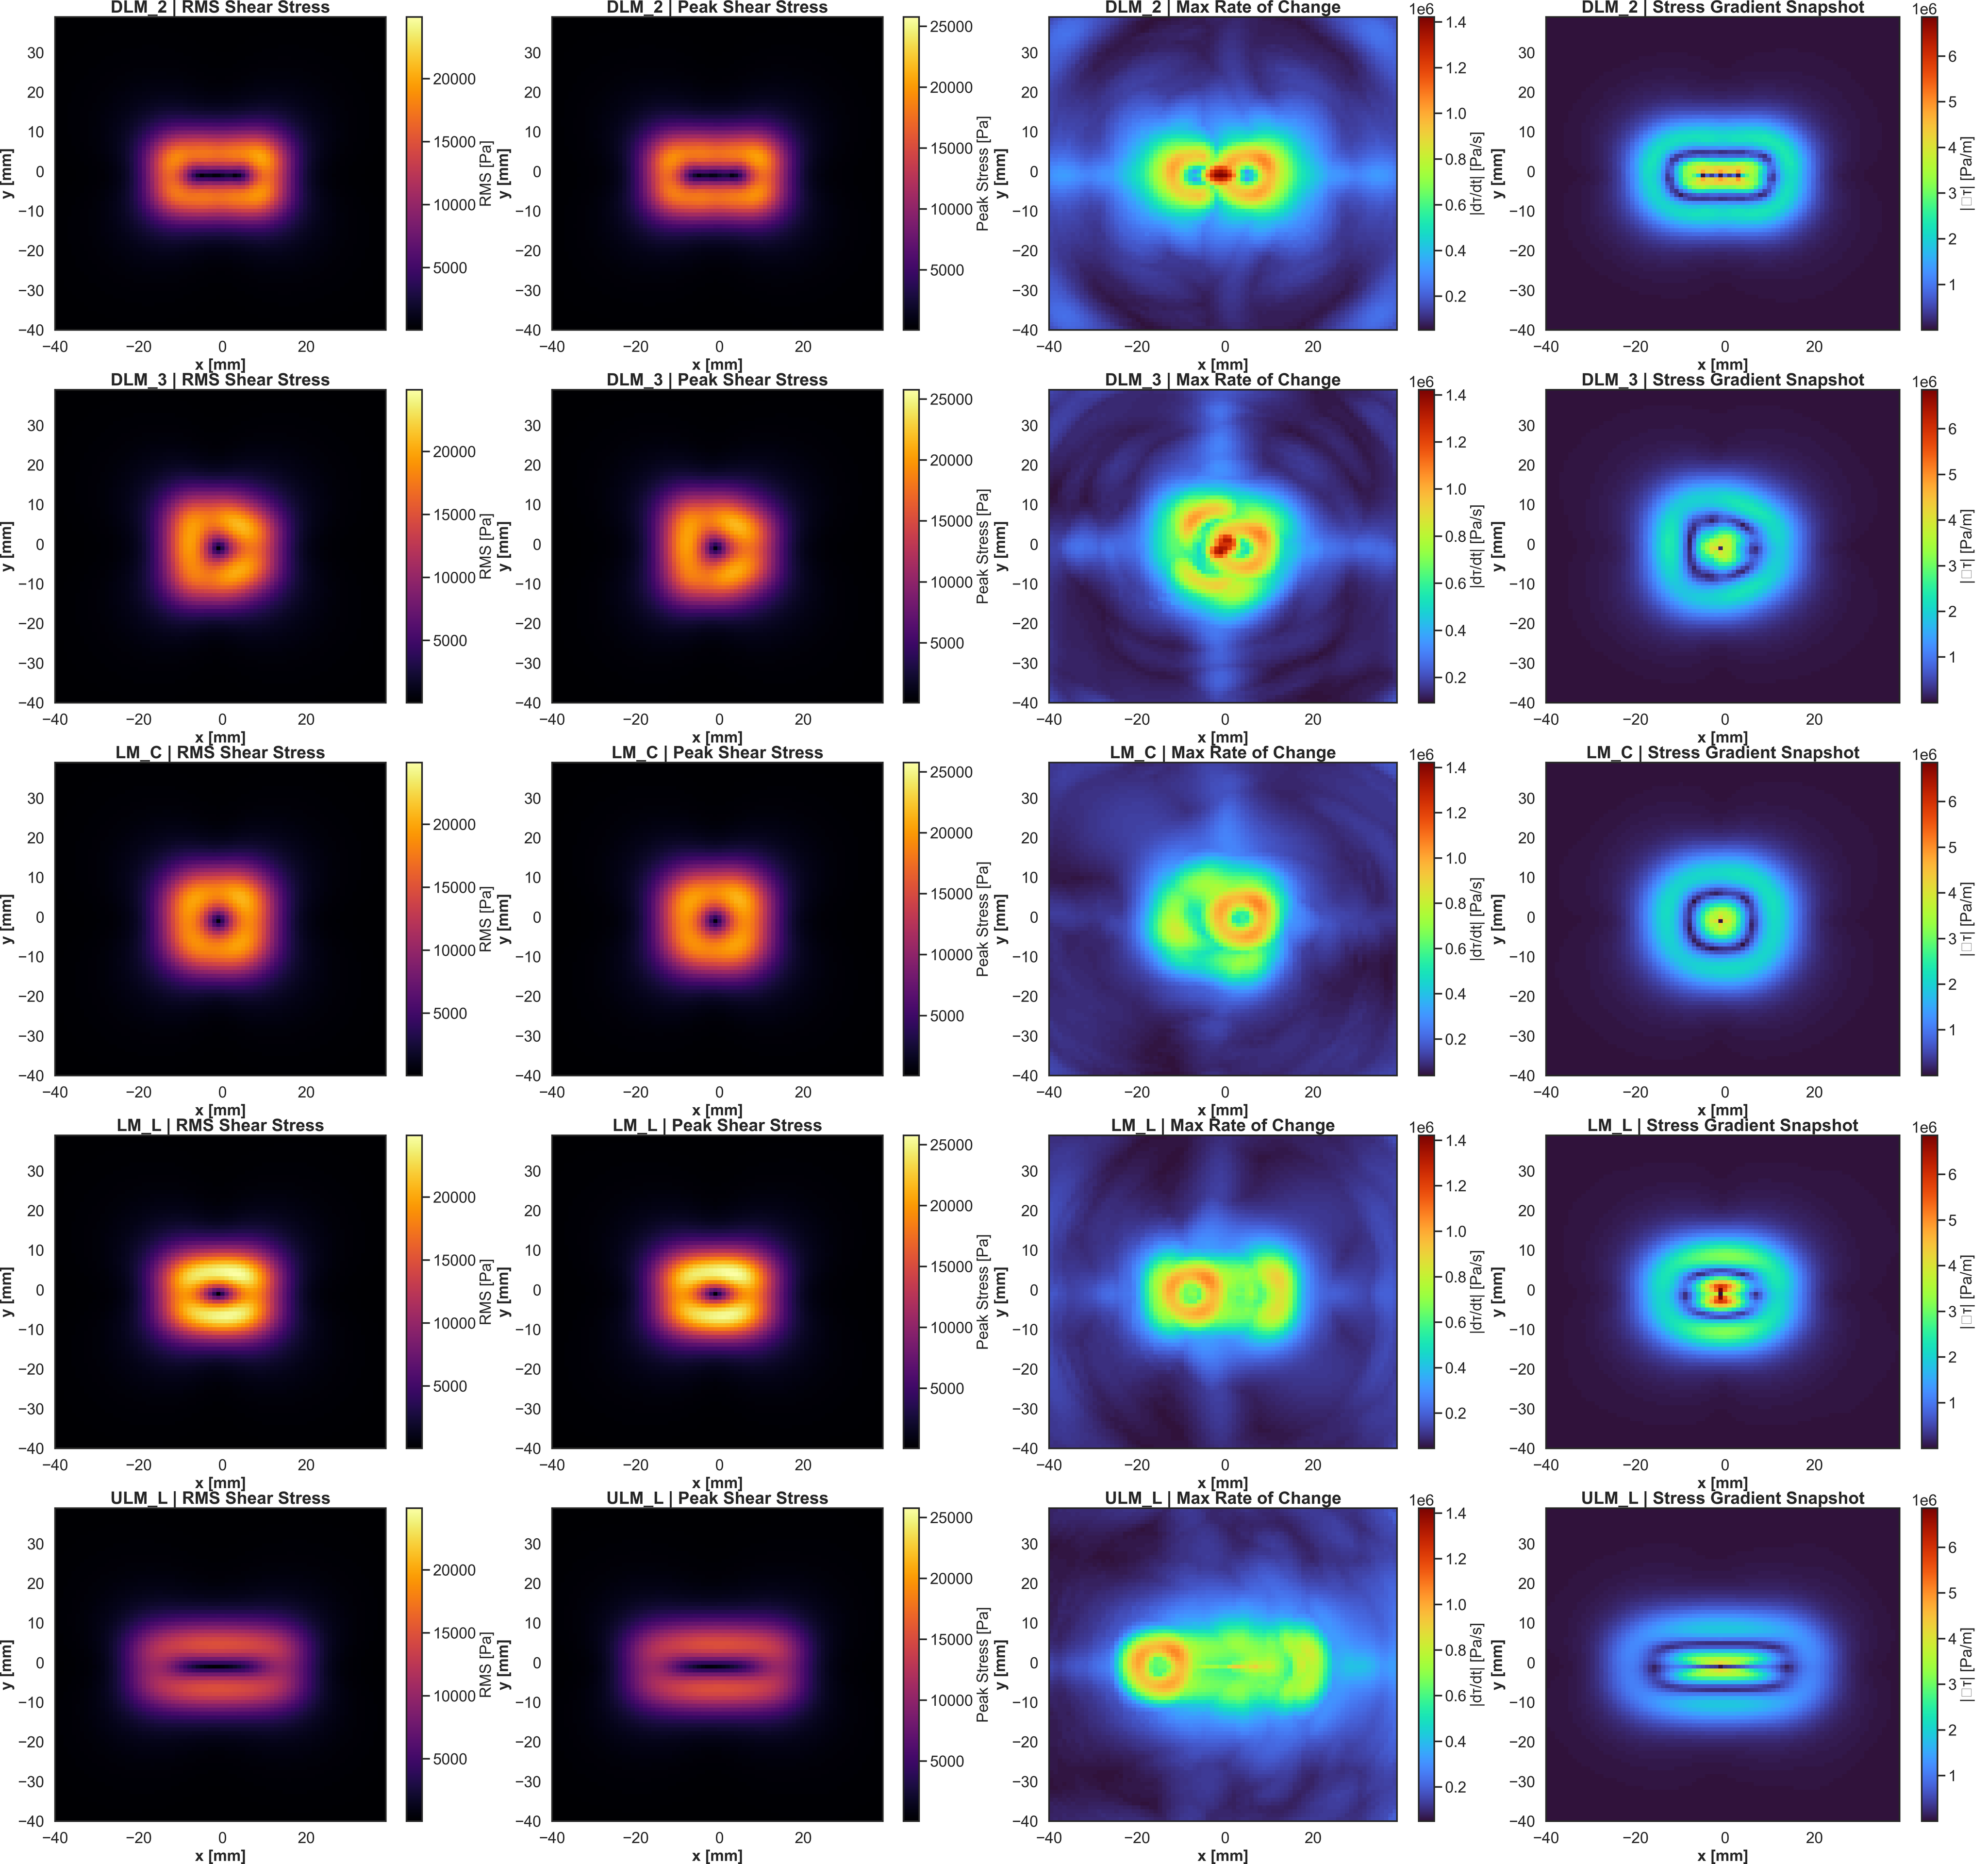
\includegraphics[width= \textwidth]{Figure_Sim_1_Full_Spatial.png}
    \caption{\textbf{Spatial distribution of stress metrics for different modulation schemes.} The rows correspond to the five modulation methods: DLM-2, DLM-3, LM-C, LM-L, and ULM-L. The columns display, from left to right: (1) \textbf{RMS Shear Stress}: The root-mean-square magnitude of the shear stress, indicating the time-averaged energy distribution. (2) \textbf{Peak Shear Stress}: The maximum instantaneous stress magnitude recorded. (3) \textbf{Max Rate of Change}: The maximum time derivative of the stress ($\max |d\boldsymbol{\tau}/dt|$), representing the dynamic impact intensity. (4) \textbf{Stress Gradient Snapshot}: A snapshot of the spatial stress gradient magnitude ($|\nabla \boldsymbol{\tau}|$), reflecting the spatial sharpness of the stimulus. All metrics are evaluated at a depth of \qty{1}{\milli\meter}.}
    \label{fig:supplementary_figure_sim_1_full_spatial}
\end{figure}

\begin{figure}[htbp]
    \centering
    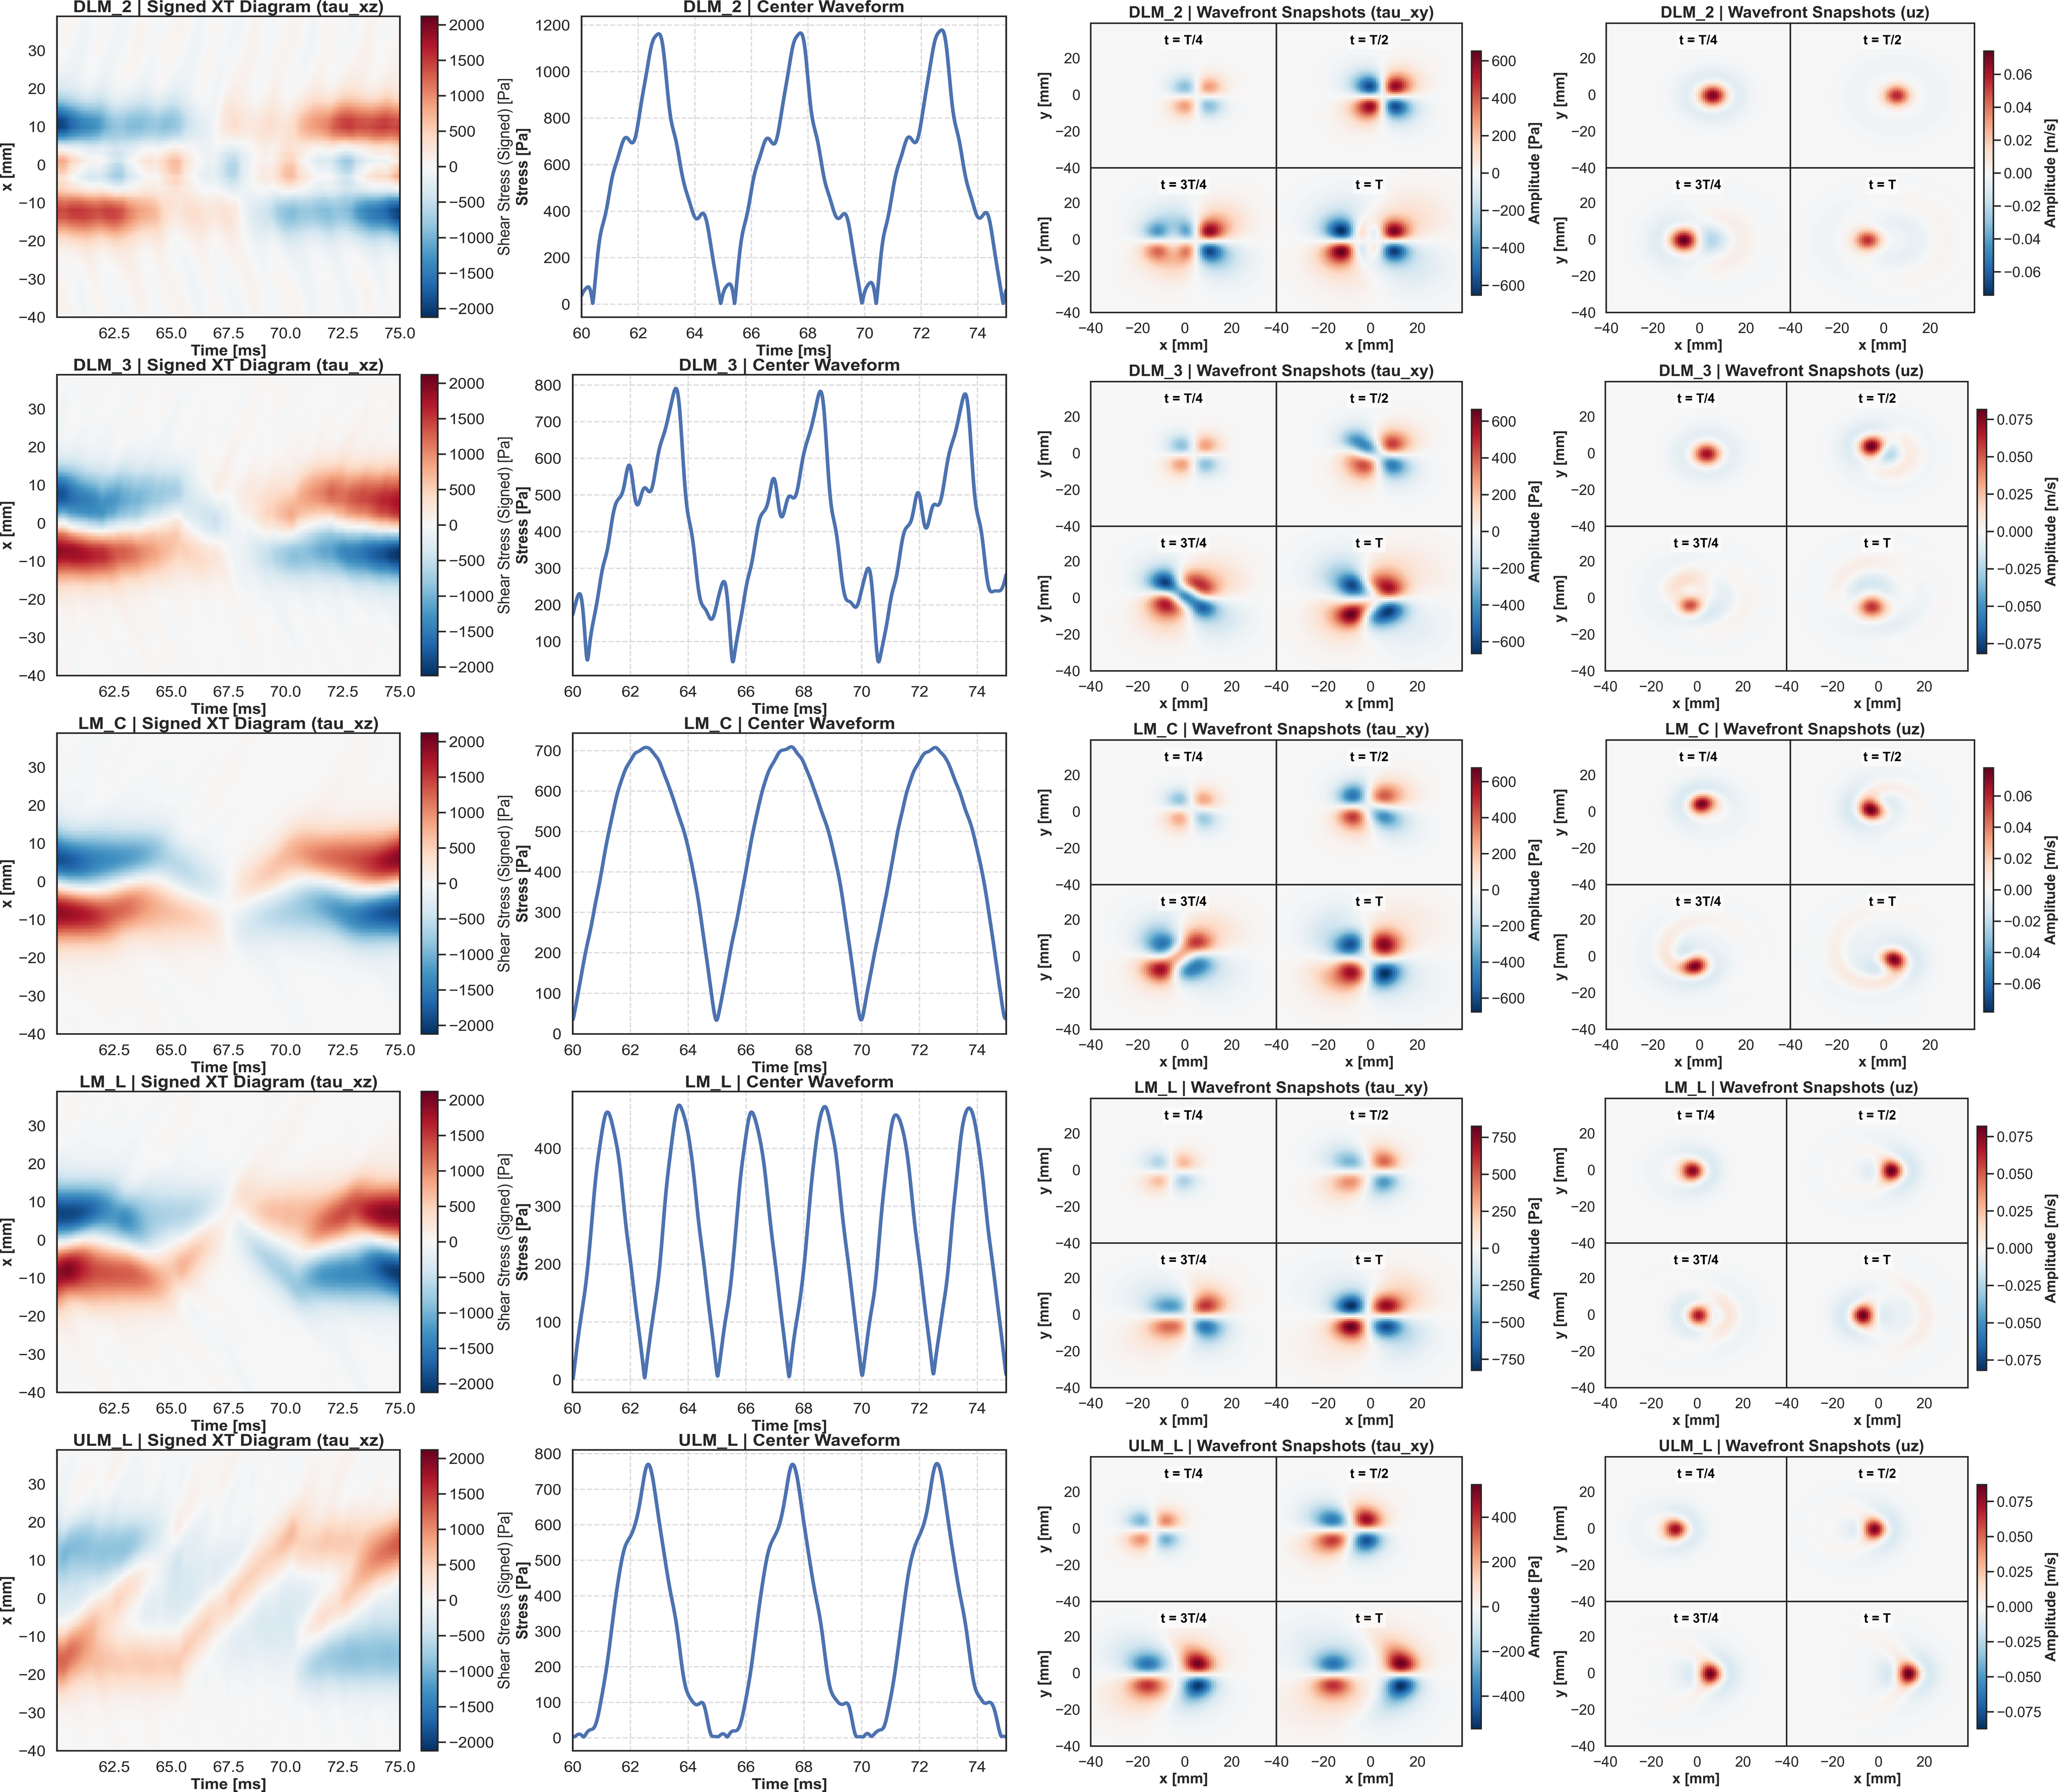
\includegraphics[width= \textwidth]{Figure_Sim_1_Full_Tempo.png}
    \caption{\textbf{Temporal evolution and wavefront dynamics.} The rows represent the modulation schemes: DLM-2, DLM-3, LM-C, LM-L, and ULM-L. The columns show: (1) \textbf{Signed XT Diagram ($\tau_{xz}$)}: Space-time plot of the shear stress component $\tau_{xz}$ along the x-axis, illustrating the wave propagation direction and interference patterns. (2) \textbf{Center Waveform}: Time history of the stress magnitude at the focal center, showing the temporal modulation envelope. (3) \textbf{Wavefront Snapshots ($\tau_{xy}$)}: Instantaneous spatial distributions of shear stress $\tau_{xy}$ at four phases ($t=T/4, T/2, 3T/4, T$) within a modulation cycle. (4) \textbf{Wavefront Snapshots ($u_z$)}: Corresponding snapshots of the vertical displacement velocity, highlighting the primary wave propagation.}
    \label{fig:supplementary_figure_sim_1_full_temporal}
\end{figure}


\SupplementarySection{Computational neural dynamics modeling details}

We developed a minimal but mechanistically grounded peripheral neural model to test whether the psychophysical ranking of the five ultrasonic modulation strategies could be explained from the dynamics of cutaneous shear-wave propagation rather than from static mechanical extrema alone. The model was tailored to the dominant vibrotactile channel expected under the present stimulation regime, namely the Pacinian-associated rapidly adapting type II pathway, because all tactile stimuli were designed around a modulation frequency of \qty{200}{\hertz}, close to the frequency range in which this channel shows maximal sensitivity in glabrous skin~\citep{mountcastleNeuralBasisSense1967, talbotSenseFluttervibrationComparison1968a, bolanowskiFourChannelsMediate1988, johnsonRolesFunctionsCutaneous2001, handlerMechanosensoryNeuronsTouch2021}. This restricted model scope was intentional. The goal was not to reconstruct the full diversity of cutaneous afferents, but to ask whether a small set of physiologically interpretable operations applied to the simulated stress fields was sufficient to reproduce the main perceptual ordering across modulation methods. We therefore kept all model parameters fixed across conditions and allowed the five modulation schemes to differ only through their input spatiotemporal mechanical fields.

The model took as input the steady-state spatiotemporal shear-stress fields obtained from the numerical wave-propagation simulations described above. For each modulation method, the recorded fields within the analysis region of interest were the three orthogonal shear components $\tau_{xy}(x,y,t)$, $\tau_{xz}(x,y,t)$, and $\tau_{yz}(x,y,t)$, sampled on a regular lattice at \qty{1}{\milli\meter} depth below the surface. We used the steady-state window rather than the full stimulus epoch because the psychophysical comparison focused on the sustained percept generated during ongoing stimulation, and because this window isolates the modulation-specific propagation pattern after initial transients had decayed. In accordance with the design logic of the model, we did not feed summary descriptors such as RMS stress, peak stress, Frequency Fidelity Index, or Directional Wavefront Concentration Index into the neural simulation. Those quantities remained external diagnostic measures. The neural model operated directly on the underlying fields so that any ranking would emerge from the field dynamics themselves rather than from hand-crafted scalar features.

A lattice of virtual receptors was then placed across the region of interest with uniform spatial spacing of \qty{2}{\milli\meter}. This receptor lattice covered the same physical extent for every modulation method and provided a common substrate for comparing population responses. Let $r_i=(x_i,y_i)$ denote the position of receptor $i$, and let $r_j=(x_j,y_j)$ denote the location of source sample $j$ in the simulated field. For each of the three shear components, we first removed the static bias by subtracting the temporal mean at every spatial point,
\begin{equation}
\tau^{\mathrm{dyn}}_{c}(r_j,t)=\tau_{c}(r_j,t)-\langle \tau_{c}(r_j,\cdot)\rangle_t,
\end{equation}
where $c \in \{xy,xz,yz\}$. This step reflects the well-established property that Pacinian-associated responses are driven predominantly by dynamic vibration and transients rather than by static indentation~\citep{johanssonTactileSensoryCoding1983, johnsonRolesFunctionsCutaneous2001, handlerMechanosensoryNeuronsTouch2021}. It also aligns the model with recent evidence that the Pacinian inner core is specialized for transient mechanical signaling~\citep{ziolkowskiInnerCoreEnables2025}.

The central operation of the model was a causal spatiotemporal integration step intended to represent the effective summation of cutaneous surface-wave inputs that arrive at a receptor after finite propagation delay. For receptor $i$ and shear component $c$, the mechanical drive was defined as
\begin{equation}
 m_{c,i}(t)=\sum_{j \in \Omega_i} K(d_{ij})\,\tau^{\mathrm{dyn}}_{c}\!\left(r_j, t-\frac{d_{ij}}{c_s}\right),
\end{equation}
with
\begin{equation}
 d_{ij}=\lVert r_j-r_i \rVert,
 \qquad
 K(d_{ij})=\exp\!\left(-\frac{d_{ij}}{\lambda}\right).
\end{equation}
Here $c_s=\qty{5}{\meter\per\second}$ was the cutaneous shear-wave speed used throughout the mechanical simulations, and $\lambda=\qty{4}{\milli\meter}$ set the spatial decay length of the integration kernel. The summation domain $\Omega_i$ comprised all source locations in the region of interest. This formulation embodies the key conceptual claim of the study: if a modulation strategy organizes the wavefront so that mechanically relevant disturbances arrive at a receptor with compatible timing, those inputs add constructively after propagation delay; if the modulation introduces repeated direction reversal, frequency doubling, or phase fragmentation, the effective drive is reduced because delayed components are less aligned. In that sense, the integral provides an explicit operational definition of coherent integration. The use of an exponentially decaying kernel is also consistent with the idea that the Pacinian channel pools vibration over a broad, but not unlimited, spatial extent~\citep{loewensteinMechanicalTransmissionPacinian1966, verrilloEffectContactorArea1963, saalSimulatingTactileSignals2017}.

We treated the contribution of the Pacinian inner core, including the combined mechanical preprocessing performed by the lamellar structure and its associated terminal elements, as part of this effective integration operator rather than as a separate multi-compartment cellular subsystem. This simplification was necessary because parameter values for a detailed human palmar Pacinian corpuscle model under ultrasonic surface-wave stimulation remain unavailable. A more elaborate representation would therefore introduce degrees of freedom that could not be independently constrained by the available data. The present formulation instead follows a principle of physiological parsimony: it preserves the experimentally grounded functions that matter most for the current question, namely transient enhancement, spatial summation, and frequency-dependent sensitivity, while avoiding unsupported microscopic assumptions~\citep{loewensteinMechanicalTransmissionPacinian1966, quindlenMultiphysicsModelPacinian2016, ziolkowskiInnerCoreEnables2025}.

The delayed mechanical drive for each component was then passed through a fixed band-pass filter representing the frequency tuning of the Pacinian-dominant channel,
\begin{equation}
 u_{c,i}(t)=(h_{\mathrm{PC}} * m_{c,i})(t),
\end{equation}
where $h_{\mathrm{PC}}$ denotes a fourth-order Butterworth band-pass filter with cutoff frequencies at \qty{150}{\hertz} and \qty{300}{\hertz}. The filter was centered on the \qty{200}{\hertz} modulation band but was deliberately not made excessively narrow. This choice preserved a physiologically plausible sensitivity profile: the Pacinian pathway is most sensitive around this range, yet it still responds over a broader band of vibration frequencies~\citep{mountcastleNeuralBasisSense1967, talbotSenseFluttervibrationComparison1968a, bolanowskiFourChannelsMediate1988, johnsonRolesFunctionsCutaneous2001}. This stage was critical for testing the hypothesis that frequency fidelity, rather than total mechanical energy alone, governs perceptual effectiveness. In practical terms, it penalized modulation schemes whose local mechanical drive shifted substantial power into non-optimal harmonics, such as the strong \qty{400}{\hertz} component expected for bidirectional linear scanning and the higher-order harmonic contamination introduced by multi-point discrete switching.

Each filtered drive $u_{c,i}(t)$ was next converted into a spike train using a leaky integrate-and-fire element,
\begin{equation}
\tau_m\frac{dV_{c,i}}{dt}=-V_{c,i}+g\,[u_{c,i}(t)]_{+},
\end{equation}
with membrane time constant $\tau_m=\qty{2}{\milli\second}$, absolute refractory period $t_{\mathrm{ref}}=\qty{2}{\milli\second}$, threshold $V_{\mathrm{th}}=1$, and a common gain factor $g=1$. When $V_{c,i}(t)$ reached threshold, the unit emitted one spike, the membrane state was reset, and the unit remained inactive during the refractory interval. We used this simple fast-adapting spiking model because it captures the two response properties most relevant to the present problem, namely sensitivity to temporally filtered dynamic input and capacity for phase-locked repetitive firing, while avoiding unnecessary parameterization. We did not use method-specific gains or thresholds. All five modulation methods therefore traversed the same neural nonlinearity.

For each receptor and each shear component, we quantified the steady-state response by combining firing rate and phase locking to the intended modulation frequency. If receptor $i$ generated spikes at times $\{t_k\}_{k=1}^{N_i}$ for component $c$, the vector strength at \qty{200}{\hertz} was computed as
\begin{equation}
VS_{c,i}=\left|\frac{1}{N_i}\sum_{k=1}^{N_i} \exp\!\left(\mathrm{i}2\pi f_0 t_k\right)\right|,
\end{equation}
with $f_0=\qty{200}{\hertz}$. Let $r_{c,i}$ denote the corresponding steady-state firing rate. We then defined a component-specific effective coding weight,
\begin{equation}
 w_{c,i}=r_{c,i}\,VS_{c,i}.
\end{equation}
This metric assigns high weight only to receptors that not only fire strongly, but also remain temporally aligned with the target modulation period. We used vector strength because the proposed mechanism predicts that perceptually effective stimuli should preserve a coherent \qty{200}{\hertz} temporal structure at the neural level, not merely elevate total spike count.

The three orthogonal shear channels were combined at each receptor by a directional max-pooling rule,
\begin{equation}
 w_i=\max\left(w_{xy,i},w_{xz,i},w_{yz,i}\right).
\end{equation}
This operation avoids imposing an a priori preferred shear direction on the receptor population. Instead, it assumes that the relevant local drive is dominated by the shear component that is most effectively converted into phase-locked firing at that receptor. This choice was motivated by the fact that the five modulation schemes differ substantially in the orientation and evolution of their local wavefronts. A scalar equivalent-stress compression at the outset would lose that directional structure, whereas max pooling retains sensitivity to whichever component best expresses the local mechanically effective mode.

The population intensity score for modulation method $m$ was then defined as
\begin{equation}
 S^{(m)}_{\mathrm{intensity}}=\log\!\left(1+\sum_i w_i\right).
\end{equation}
The logarithmic compression prevents the final metric from being dominated by a small number of exceptionally active receptors and approximates a saturating population readout. Because the same readout was applied to all methods, differences in $S_{\mathrm{intensity}}$ directly reflect differences in how efficiently each modulation pattern generates spatially distributed, phase-locked, fast-adapting activity in the Pacinian-dominant pathway. Importantly, the model does not encode any explicit label indicating whether the input came from $DLM_2$, $DLM_3$, $ULM_L$, $LM_L$, or $LM_C$. Any ordering among methods must therefore arise from the interaction between the field dynamics and the fixed neural operators.

To compare the model with the paired-comparison psychophysics, we transformed the five population intensity scores into standardized values,
\begin{equation}
\hat{S}^{(m)}=\frac{S^{(m)}_{\mathrm{intensity}}-\mu_S}{\sigma_S},
\end{equation}
where $\mu_S$ and $\sigma_S$ are the mean and standard deviation of the five method scores. For any two methods $A$ and $B$, the predicted probability that $A$ would be preferred over $B$ in the intensity task was then written as
\begin{equation}
P(A \succ B)=\frac{1}{1+\exp\left[-\left(\hat{S}^{(A)}-\hat{S}^{(B)}\right)\right]}.
\end{equation}
This mapping introduced only a common monotonic decision function and no method-specific fitting parameters. The model therefore remained generative in the limited sense intended here: it produced an ordering and pairwise preference structure from first-principles-inspired processing of the simulated wave fields, rather than by regressing directly onto the psychophysical observations.

The resulting model output reproduced the principal ranking observed in the behavioral data. The standardized neural intensity score was highest for $ULM_L$ ($z=1.196$), followed by $DLM_2$ ($z=0.634$), $DLM_3$ ($z=0.079$), $LM_C$ ($z=-0.135$), and $LM_L$ ($z=-1.773$). The corresponding pairwise probabilities showed a strong predicted advantage of $ULM_L$ over $LM_L$ ($P=0.951$) and over $LM_C$ ($P=0.791$), as well as a marked disadvantage of $LM_L$ relative to every other method. This pattern is notable because it emerged even though the model did not use static stress maxima, geometric focusing width, or experimentally measured preference scores as inputs. Instead, the ranking followed from three interacting principles: constructive delayed summation of propagating shear waves, preferential transmission of the \qty{200}{\hertz} band, and nonlinear conversion into phase-locked fast-adapting spikes.

Mechanistically, the model explains why $ULM_L$ can outperform conditions with larger local mechanical extrema. In the unidirectional linear scan, the wavefront is advanced continuously in one direction at a speed close to the simulated surface-wave speed, which favors repeated arrival of mechanically relevant components with compatible delay structure. At the same time, the scan preserves the intended \qty{200}{\hertz} stimulus rhythm at a local point, so the delayed mechanical drive remains well aligned with the Pacinian band-pass filter and supports phase-locked firing. By contrast, $LM_L$ repeatedly reverses direction and traverses the same central region twice per modulation cycle, which generates strong \qty{400}{\hertz}-like periodicity and disrupts directional continuity. In the model, these properties jointly reduce the filtered drive and degrade coherent spike timing, yielding the lowest population score. $DLM_2$ occupies an intermediate but favorable regime because appropriately timed switching between two discrete points can still create strong delayed coincidence at the receptor level while introducing less harmonic contamination than the three-point discrete condition. $DLM_3$ and $LM_C$ generate more rotationally distributed wave organizations that remain effective, but they disperse mechanically useful energy across more complex directional or harmonic structures and therefore do not achieve the same population gain as $ULM_L$.

Taken together, this computational neural dynamics model provides a compact mechanistic bridge between the elastic-wave simulations and the psychophysical paired-comparison results. It supports the interpretation that tactile efficacy in ultrasonic haptics is governed not by static local maxima alone, but by whether the modulation pattern delivers mechanically relevant energy to the Pacinian-dominant pathway in a temporally faithful and propagationally coherent form. In this framework, frequency fidelity and spatiotemporal coherence are not abstract descriptive labels. They become explicit computational requirements for generating strong, phase-locked afferent population responses under weak airborne ultrasonic stimulation~\citep{reardonCutaneousWavePropagation2019, reardonShearShockWaves2023, saalSimulatingTactileSignals2017}.

\bibliography{SWIM}% common bib file

\end{document}
